\documentclass{article}
\usepackage{amsmath}
\usepackage{xcolor}
\usepackage[margin=1in]{geometry}
\usepackage{graphicx}
\usepackage{mdframed}
\usepackage{float}
\usepackage{xcolor}
\usepackage{tikz}
\usepackage{amsmath}
\usepackage{pgfplots}
\pgfplotsset{compat=1.15}

\definecolor{solutionblue}{RGB}{0,0,255}
\usetikzlibrary{plotmarks}

\begin{document}

% Header
\begin{center}
    \textbf{\LARGE Assignment 8} \\[1ex]
    \textbf{ECE 360} \\[1ex]
    \textbf{V00984826} \\[2ex]
\end{center}

% Question and Solution Template

% Example Question and Solution (B-7-1, S-7-1)
\section*{B-7-9}
A system with the open-loop transfer function
\[
G(s)H(s) = \frac{K}{s^2 (T_1s + 1)}
\]
is inherently unstable. This system can be stabilized by adding derivative control. Sketch the polar plots for the open-loop transfer function with and without derivative control.

\section*{S-7-9}
The given open-loop transfer function is:
\[
G(s)H(s) = \frac{K}{s^2 (T_1s + 1)}
\]
This system is unstable because of the double pole at the origin. Introducing derivative control modifies the transfer function as follows:
\[
G(s)H(s) = \frac{K (T_2s + 1)}{s^2 (T_1s + 1)}, \quad (T_2 > T_1 > 0)
\]

Below are the Nyquist plots for the two cases:

\begin{figure}[H]
    \centering
    \begin{tikzpicture}[scale=2]
        % Axes
        \draw[->] (-3,0) -- (1,0) node[right] {$\text{Re}$};
        \draw[->] (0,-2) -- (0,2) node[above] {$\text{Im}$};
        
        % Cross and -1 label on x-axis
        \node[font=\large] at (-1,0) {$\times$};
        \node[below] at (-1,0) {$-1$};
        
        % Unstable system curve (top curve)
        \draw[thick] plot[smooth, tension=0.7] 
            coordinates {(-3,0.1) (-2,0.15) (-1.5,0.4) (-1,0.8) (-0.5,0.4) (-0.2,0.1) (0,0)};
        \node[above right] at (-1,0.8) {$G(s)H(s) = \frac{K}{s^2(T_1s+1)}$ (Unstable)};
        
        % Stable system curve (bottom curve)
        \draw[thick] plot[smooth, tension=0.7] 
            coordinates {(-3,-0.1) (-2,-0.15) (-1.5,-0.4) (-1,-0.8) (-0.5,-0.4) (-0.2,-0.1) (0,0)};
        \node[below right] at (-1,-0.8) {$G(s)H(s) = \frac{K(T_2s+1)}{s^2(T_1s+1)}$, $(T_2>T_1>0)$ (Stable)};
        
    \end{tikzpicture}
    \caption{Nyquist plots for systems with and without derivative control}
\end{figure}

\section*{B-7-16}
Consider the closed-loop system shown below. $G(s)$ has no poles in the right-half $s$ plane.

\begin{center}
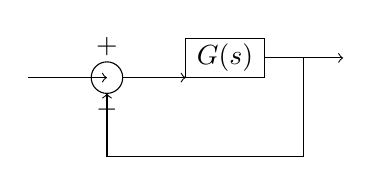
\begin{tikzpicture}
    % Draw feedback system
    \draw[->] (-2,0) -- (-1,0);
    \draw (-1,0) circle (0.2);
    \node at (-1,0.4) {$+$};
    \node at (-1,-0.4) {$-$};
    \draw[->] (-0.8,0) -- (0,0);
    \draw (0,0) rectangle (1,0.5);
    \node at (0.5,0.25) {$G(s)$};
    \draw[->] (1,0.25) -- (2,0.25);
    \draw[->] (1.5,0.25) -- (1.5,-1) -- (-1,-1) -- (-1,-0.2);
\end{tikzpicture}
\end{center}

If the Nyquist plot of $G(s)$ is as shown in Figure 7-158(a), is this system stable?

If the Nyquist plot is as shown in Figure 7-158(b), is this system stable?

\section*{S-7-16}
Let's analyze this system step by step using the Nyquist stability criterion:

1) First, recall that for a system with no poles in the right-half plane, the system is stable if and only if the Nyquist plot does not enclose the $-1+j0$ point.

2) For Figure 7-158(a):
   - The Nyquist plot does not enclose the $-1+j0$ point
   - The plot passes near but does not encircle the critical point
   - Therefore, according to the Nyquist stability criterion, the system is stable

3) For Figure 7-158(b):
   - The Nyquist plot makes one complete counterclockwise encirclement of the $-1+j0$ point
   - According to the Nyquist criterion, this means the closed-loop system has one pole in the right-half plane
   - Therefore, the system is unstable

Therefore:
- For case (a): The system is stable
- For case (b): The system is unstable
\section*{B-7-23}
Consider the unity-feedback control system whose open-loop transfer function is
\[
G(s) = \frac{as + 1}{s^2}
\]
Determine the value of $a$ so that the phase margin is $45°$.

\section*{S-7-23}
For this unity-feedback system, we need to analyze the frequency response to find the value of $a$ that gives a phase margin of $45°$.

The magnitude and phase of $G(j\omega)$ are:
\[
|G(j\omega)| = \frac{\sqrt{a^2\omega^2 + 1}}{\omega^2}
\]
\[
\angle G(j\omega) = \tan^{-1}(a\omega) - 180°
\]

At the gain crossover frequency $\omega_1$ (where $|G(j\omega_1)| = 1$), we require:
\[
\frac{\sqrt{a^2\omega_1^2 + 1}}{\omega_1^2} = 1
\]
\[
\tan^{-1}(a\omega_1) - 180° = -135° \quad \text{(for 45° phase margin)}
\]

From these conditions, we can write:
\[
a^2\omega_1^2 + 1 = \omega_1^4
\]
\[
a\omega_1 = 1
\]

Solving these equations:
\[
a = \left(\frac{1}{\sqrt{2}}\right)^{\frac{1}{2}} = 0.841
\]

Therefore, the value of $a$ that gives a phase margin of $45°$ is 0.841.
\section*{B-7-26}
Consider a unity-feedback control system with the open-loop transfer function
\[
G(s) = \frac{K}{s(s^2 + s + 4)} = \frac{0.25K}{s(0.25s^2 + 0.25s + 1)}
\]

The quadratic term in the denominator has the undamped natural frequency of 2 rad/sec and the damping ratio of 0.25. Determine the value of the gain $K$ such that the phase margin is $50°$. What is the gain margin with this gain $K$?

\section*{S-7-26}
Let's solve this step by step:

1) At frequency $\omega_1$ corresponding to $-130°$ phase (for $50°$ phase margin):
\[
\angle G(j\omega_1) = -1j\omega_1 - [1-0.25\omega_1^2 + j0.25\omega_1] = -130°
\]
\[
= -90° - \tan^{-1}\frac{0.25\omega_1}{1-0.25\omega_1^2} = -130°
\]

2) Solving this equation, we find $\omega_1 = 1.491$ rad/sec

3) At this frequency, the magnitude must be unity:
\[
|G(j1.491)| = \left|\frac{0.25K}{(j1.491)(-0.555 + j0.3725 + 1)}\right| = 0.2890K = 1
\]

4) Setting $|G(j1.491)| = 0.2890K = 1$, we find:
\[
K = 3.46
\]

5) Note that the phase crossover frequency is at $\omega = 2$ rad/sec:
\[
\angle G(j2) = -\angle j2 - \angle(-0.25x2^2+0.25xj2+1) = -90°-90° = -180°
\]

6) The magnitude $|G(j2)|$ with $K = 3.46$ becomes:
\[
|G(j2)| = \left|\frac{0.865}{(j2)(-1+0.5j+1)}\right| = 0.865 = -1.26\text{ dB}
\]

Therefore:
- The required gain $K = 3.46$
- The gain margin is 1.26 dB

\begin{figure}[h]
    \centering
    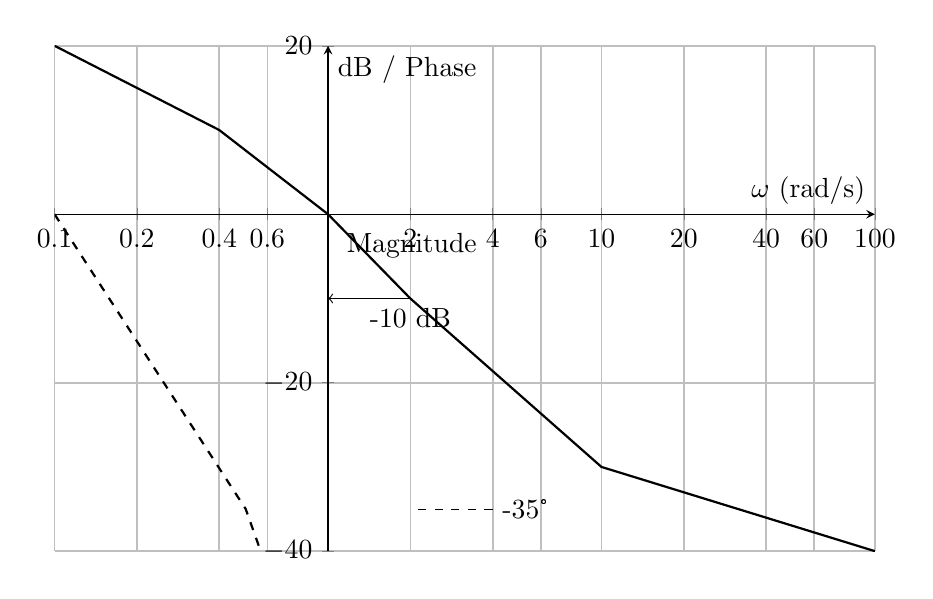
\begin{tikzpicture}
        % Axes
        \begin{axis}[
            width=12cm, height=8cm,
            xlabel={$\omega$ (rad/s)},
            ylabel={dB / Phase},
            xmin=0.1, xmax=100,
            ymin=-40, ymax=20,
            xmode=log,
            xtick={0.1, 0.2, 0.4, 0.6, 1, 2, 4, 6, 10, 20, 40, 60, 100},
            xticklabels={0.1, 0.2, 0.4, 0.6, 1, 2, 4, 6, 10, 20, 40, 60, 100},
            ytick={-40, -20, 0, 20},
            grid=both,
            major grid style={line width=0.6pt, draw=gray!50},
            minor grid style={line width=0.3pt, draw=gray!20},
            axis lines=middle,
            legend pos=south west
        ]

        % Magnitude plot
        \addplot[thick, black, mark=none] coordinates {
            (0.1, 20) (0.4, 10) (1, 0) (2, -10) (10, -30) (100, -40)
        } node[pos=0.35, below right] {Magnitude};

        % Phase plot
        \addplot[thick, dashed, black, mark=none] coordinates {
            (0.1, 0) (0.5, -35) (2, -90) (10, -180) (100, -270)
        } node[pos=0.7, below] {Phase};

        % Annotated points
        \node[below] at (axis cs:2,-10) {-10 dB};
        \draw[->] (axis cs:2,-10) -- (axis cs:1,-10);

        \node[right] at (axis cs:4,-35) {-35°};
        \draw[dashed] (axis cs:4,-35) -- (axis cs:2,-35);
        \end{axis}
    \end{tikzpicture}
    \caption{Bode plot with magnitude and phase.}
\end{figure}

\end{document}

% Question text
% EXAMPLE TEXT
% Insert question image if needed
%\begin{center}
%    \includegraphics[width=0.8\textwidth]{image_B-7-1} % Replace "image_B-7-1" with the actual filename
%\end{center}
%The following MATLAB program produces the Bode diagram shown below.
%
%\begin{mdframed}
%{\color{solutionblue}
%\begin{verbatim}
%% ***** Bode diagram *****
%num = [0 10 4 10];
%den = [1 0.8 9 0];
%bode(num, den)
%title('Bode Diagram of G(s) = 10(s^2 + 0.4s + 1)/[s(s^2 + 0.8s + 9)]')
%\end{verbatim}}
%\end{mdframed}
%\begin{figure}[H]
%    \centering
%    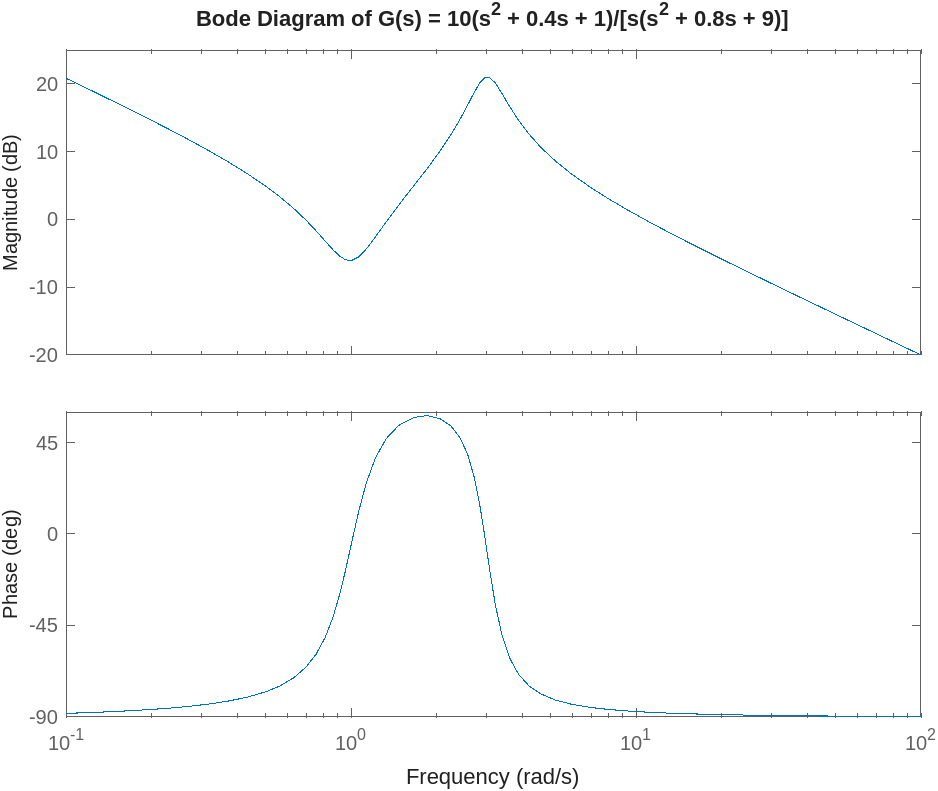
\includegraphics[width=0.85\textwidth]{/Users/arfaz/Desktop/ThirdYearEngineering/2 Fall 2024/1 ECE 360 A01 B05/1 Q-As/MatLab Files/A7/ECE360-B-7-4.png}
%    \caption{Bode Diagram of \( G(s) = \frac{10(s^2 + 0.4s + 1)}{s(s^2 + 0.8s + 9)} \)}
%\end{figure}